\documentclass[11pt]{scrartcl}
\usepackage{dominatrix}

\usepackage{colortbl}
\usepackage{pgfplots}
\newcommand{\jon}{Jón }
\newcommand{\ve}{\varepsilon}
\pgfplotsset{compat=1.9}
\renewcommand\thesubsection{\alph{subsection}}
\definecolor{light-gray}{gray}{0.75}
\title{Consumption Savings}
\subject{ECON W3213 Spring 2014 \jon Steinsson}
\author{Linan Qiu, lq2137}
\begin{document}

\maketitle

\begin{abstract}
This set of recitation notes covers \textbf{Consumption and Savings} This is in no way a substitute for attending lectures, but just in case you dozed off or checked your boyfriend's Facebook page while \jon was working Calculus magic on the board, this set of notes may save you.
\end{abstract}

\section{Consumption Savings Model}

Let's suppose that you only live in two periods, 1 and 2. Sad you.

\subsection{Utility Function}

Your utility function is then

\[ U(C_1) + \beta U(C_2)\]

where $C_1$ is your consumption in period 1, and $C_2$ is your consumption in period 2. $\beta$ is a discounting factor. If $\beta$ is less than 1, then you value future consumption less than present consumption of the same amount.

\subsection{Budget Constraint}

\[C_1 + B = Y_1\]

Whatever you earn in period 1, $Y_1$, is either consumed, $C_1$, or saved $B$. $B$ is positive when you save. However, when you borrow, $B$ is negative.

\[C_2 = Y_2 + (1+R)B \]

In the second period, you earn $Y_2$. If you saved in 1, then you will be able to consume $C_2$ everything you earned $Y_2$, plus whatever you saved with interest $(1+R)B$. However, if you borrowed, $B$ will be negative, and it subtracts away from $Y_2$, leaving you to consume less than you earned in $Y_2$.

$B$ has the following constraints

\begin{itemize}
\item $B < Y_1$, since you can't save more than you earn
\item $-(1+R)B < Y_2$, since the amount you borrow, with interest, can't be more than what you earn in period 2. Otherwise, you won't be able to pay back! This implies that $B > -\frac{Y_2}{1+R}$
\end{itemize}

We can combine the two equations to form our constraint 

\[ C_1 + \frac{C_2}{1+R} = Y_1 + \frac{Y_2}{1+R} \]

On the left, we have the present value of total consumption throughout all periods. On the right, it's the present value of income throughout all periods. For a detailed explanation of present value, look at the \href{https://github.com/linanqiu/econ-w3213-recitation-notes/blob/master/00\%20Mathematics\%20Crash\%20Course.pdf?raw=true
}{00 Mathematics Crash Course.pdf} notes.

\subsection{Maximizing Utility}

We have the utility function

\[ U(C_1) + \beta U(C_2)\]

subject to the constraint

\[ C_1 + \frac{C_2}{1+R} = Y_1 + \frac{Y_2}{1+R} \]

We rewrite the constraint as in terms of $C_2$ so that we can plug it into the utility function

\[ C_2 = Y_1 (1+R) + Y_2 - C_1 (1+R) \]

\begin{align*}
\frac{\partial}{\partial C_1} \left[ U(C_1) + \beta U(C_2) \right] &= \frac{\partial}{\partial C_1} \left[ U(C_1) +  \beta U(Y_1 (1+R) + Y_2 - C_1 (1+R)) \right] \\
&= U'(C_1) - (1+R)\beta U'(Y_1 (1+R) + Y_2 - C_1 (1+R)) \\
&=  U'(C_1) - (1+R)\beta U'(C_2) = 0 \\
\frac{U'(C_1)}{U'(C_2)} &= (1+R)\beta 
\end{align*}

This is the \textbf{Consumption Euler Equation}

Let's make intuitive sense of this animal.

\begin{itemize}
\item $U'(C_1)$ is the additional utility of consuming an additional unit in period 1
\item $-\beta (1+R) U'(C_2)$ is the partial derivative of $U(C_2)$ with respect to $C_1$. Intuitively, this means that if I consume an additional unit in period 1, I will lose $\beta (1+R) U'(C_2)$ utility in period 2.
\item These two should be equal to maximize utility. Think marginal benefit and costs.
\end{itemize}

\section{Consumption Growth}

\subsection{Specific Utility Function}

Let's plug in a specific function for the utility to yield more insights. As usual, we use 

\[U(C) = \log{C} \]

Why? Because this function is increasing at a decreasing rate. Or you can call it concave. Verify for yourself that the first order derivative is positive and the second order derivative is negative.

With that,

\[U'(C) = \frac{1}{C} \]

Then,

\begin{align*}
\frac{U'(C_1)}{U'(C_2)} &= (1+R)\beta  \\
\frac{C_2}{C_1} &= (1+R) \beta 
\end{align*}

$\frac{C_2}{C_1}$ is the growth rate of consumption. Hence, we find that consumption growth is \textbf{completely independent of income growth}. Why do you do that? Well, since you know how much income you're going to make throughout your life, you'd want to average out your consumption. Hence, your consumption is going to be independent of your change in income. It is only going to reflect your life's income.

\subsection{Level of Consumption}

We can express future consumption in terms of present consumption and $\beta$

\[ C_2 = C_1 (1+R) \beta \]

Plugging this into our budget constraint, we get

\begin{align*}
C_1 + \frac{C_2}{1+R} &= Y_1 + \frac{Y_2}{1+R} \\
C_1 + \frac{C_1 (1+R) \beta}{1+R} &= Y_1 + \frac{Y_2}{1+R} \\
C_1 (1 + \beta) &= Y_1 + \frac{Y_2}{1+R} \\
C_1 &= \frac{1}{1+\beta} \left(Y_1 + \frac{Y_2}{1+R}\right)
\end{align*}

We can get two conclusions

\begin{itemize}
\item Level of consumption does not depend on level of period specific income, only total income.
\item Level of consumption is a fraction, $\frac{1}{1+\beta}$, of the present value of income
\end{itemize}

\subsection{Permanent Income Hypothesis}

Let's try extending our model to 3 periods

\[ C_1 + \frac{C_2}{(1+R)} + \frac{C_3}{(1+R)^2} = Y_1 + \frac{Y_2}{(1+R)} + \frac{Y_3}{(1+R)^2} \]

We also have

\begin{align*}
\frac{C_2}{C_1} &= \beta (1+R) \\
\frac{C_3}{C_2} &= \beta (1+R)
\end{align*}

With a little bit of algebra magic, we can express everything in terms of $C_1$

\begin{align*}
C_1 + \beta C_1 + \beta^2 C_1 &=  Y_1 + \frac{Y_2}{(1+R)} + \frac{Y_3}{(1+R)^2} \\
C_1 (1+\beta + \beta^2) &=  Y_1 + \frac{Y_2}{(1+R)} + \frac{Y_3}{(1+R)^2}\\
C_1 &= \left(\frac{1}{1+\beta + \beta^2}\right) \left(Y_1 + \frac{Y_2}{(1+R)} + \frac{Y_3}{(1+R)^2}\right)
\end{align*}

We can generalize this to $n$ periods

\[ C_1 = \frac{1}{\sum\limits_{t=1}^{n} \left( \beta^{n-1} \right)} \sum\limits_{t=1}^{n}\left[ \left( \frac{1}{1+R}\right)^{t-1} Y_t \right] \] 

Now let's assume that the average person works 45 years in his life, and to make our life even easier, we assume $\beta = 1$

Then,

\[ C_1 = \frac{1}{45} \sum\limits_{t=1}^{45}\left[ \left( \frac{1}{1+R}\right)^{t-1} Y_t \right] \]

Again, our two conclusions stand true

\begin{itemize}
\item Level of consumption does not depend on level of period specific income, only total income.
\item Level of consumption is a fraction of the present value of life time income
\end{itemize}

Basically, this means that your consumption level should be independent of your income at a particular time. It is only dependent on the level of your total income over your lifetime.

\begin{figure}[H]
\begin{subfigure}[b]{0.5\textwidth}
\centering
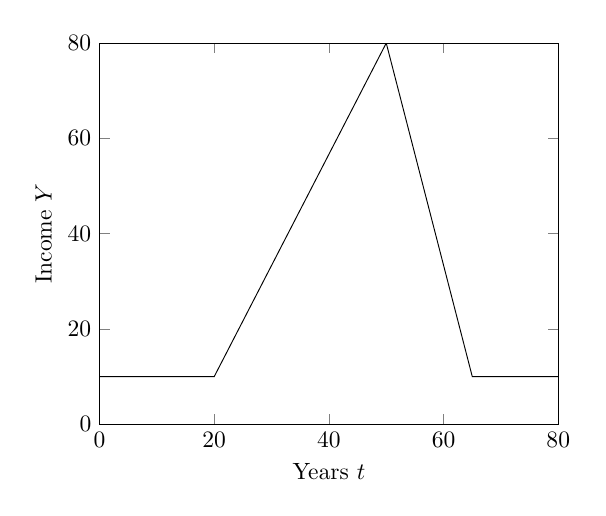
\begin{tikzpicture}[scale=0.85]
\begin{axis}[ylabel = {Income $Y$}, xlabel = {Years $t$}, xmin = 0, xmax = 80,ymin = 0, ymax = 80]

\addplot[black, domain=0:80]
coordinates{(0,10) (20,10) (50, 80) (65,10) (80,10)};

\end{axis}
\end{tikzpicture}
\end{subfigure}
\hspace{2ex}
\begin{subfigure}[b]{0.5\textwidth}
\centering
\begin{tikzpicture}[scale=0.85]
\begin{axis}[ylabel = {Consumption $C$}, xlabel = {Years $t$}, xmin = 0, xmax = 80,ymin = 0, ymax = 80]

\addplot[blue, domain=0:80]
coordinates{(0,26.875) (80, 26.875)};

\end{axis}
\end{tikzpicture}
\end{subfigure}
\caption{Income and Consumption Level throughout Lifetime}
\end{figure}

How exactly will you be able to achieve that? You borrow and you save (and pay back the loans), then you eat off those savings!

\begin{figure}[H]
\centering
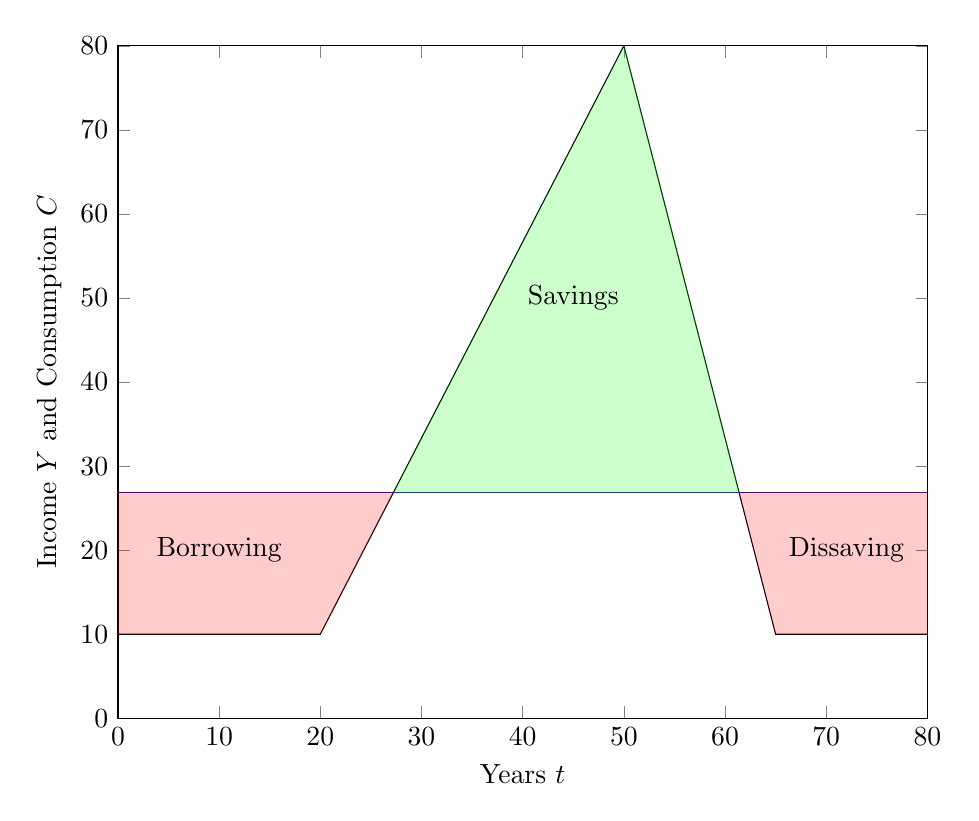
\begin{tikzpicture}
\begin{axis}[ylabel = {Income $Y$ and Consumption $C$}, xlabel = {Years $t$}, xmin = 0, xmax = 80,ymin = 0, ymax = 80, scale=1.5]

\addplot[black, domain=0:80]
coordinates{(0,10) (20,10) (50, 80) (65,10) (80,10)};

\addplot[blue, domain=0:80]
coordinates{(0,26.875) (80, 26.875)};

\addplot[fill, red, opacity = 0.2]
coordinates{(0,10) (20,10) (27.2322,26.875) (0, 26.875)};

\addplot[fill, red, opacity = 0.2]
coordinates{(65,10) (80,10) (80,26.875) (61.3839, 26.875)} ;

\addplot[fill, green, opacity = 0.2]
coordinates{(27.2322,26.875) (61.3839, 26.875) (50,80)};

\addplot[black, domain=0:80]
coordinates{(0,0)} node at (axis cs: 45, 50) {Savings} node at (axis cs: 10, 20) {Borrowing} node at (axis cs: 72, 20) {Dissaving};

\end{axis}
\end{tikzpicture}
\end{figure}

However, in reality, that doesn't happen because we have borrowing constraints.

\end{document}